\documentclass[11pt]{article}

% ---------------------------------------------------------------------
% Packages
% ---------------------------------------------------------------------
\usepackage[margin=1in]{geometry}
\usepackage[T1]{fontenc}
\usepackage{lmodern}
\usepackage{graphicx}      % \includegraphics for the figures
\usepackage{booktabs}      % \toprule, \midrule, \bottomrule in Table 1
\usepackage{caption}
\usepackage{subcaption}    % (a)/(b)/(c) panels in Figures 1--3
\usepackage{float}         % [H] placement option
\usepackage{amsmath}
\usepackage[numbers,sort&compress]{natbib}
\usepackage[hidelinks]{hyperref}

\captionsetup{font=small, labelfont=bf}
\graphicspath{{figures/}}

% Put your public GitHub repository link here
\newcommand{\repourl}{https://github.com/YOUR-USERNAME/YOUR-REPO}

\title{Early-Pregnancy Blood Gene Expression, Maternal Vitamin~D Status, and Preeclampsia}
\author{Jason Spino\\[2pt] \small QBS 103 Final Project, Fall 2026}
\date{November 11, 2026}

\begin{document}
\maketitle

% =====================================================================
\section{Methods}
% =====================================================================

\subsection{Data source}
Data come from a nested case-control study within the Vitamin D Antenatal
Asthma Reduction Trial (VDAART), described by Mirzakhani et
al.~\cite{mirzakhani2016} and deposited in the Gene Expression Omnibus as
series GSE85307~\cite{geo_gse85307}. Peripheral blood was collected at 10 to
18 weeks of gestation, and RNA was profiled on the Affymetrix Human Gene 1.0 ST
array. The initial dataset contained 157 women, 47 of whom later developed
preeclampsia and 110 of whom had a normal pregnancy. Three files were used: a
covariate file, an expression matrix with one row per array probe and one
column per sample, and a linker file matching probe IDs to gene names. Samples
were matched between files using the GEO sample ID (geoID), and the match was
checked to confirm that the expression and covariate files contained exactly
the same 157 samples.

\subsection{Final sample size}
No covariate had missing values and every probe matched a gene name, so no
samples were excluded. The final sample size was 157 women (110 normal, 47
preeclampsia).

\subsection{Variables}
Three genes were studied in detail: \textit{RUNDC3A}, \textit{LYN}, and
\textit{IGFBP1}. The continuous covariate was maternal body mass index (BMI,
kg/m$^2$). The two categorical covariates were pregnancy outcome (normal or
preeclampsia) and maternal vitamin~D status, which was derived from baseline
25-hydroxyvitamin~D. Women with 25-hydroxyvitamin~D below 20~ng/mL were
classified as deficient and the rest as sufficient. Two further continuous
covariates, maternal age and gestational age at delivery, were included in the
summary statistics table.

\subsection{Analyses}
Participant characteristics were summarised by pregnancy outcome (Table~\ref{tab:summary}).
Continuous covariates are shown as mean (SD) and were compared with Welch
two-sample $t$-tests. Vitamin~D status is shown as $n$ (\%) and was compared
with a chi-squared test with continuity correction.

For each gene, a histogram showed the distribution of expression, a
scatterplot with a least-squares line showed expression against maternal BMI
(summarised by the Pearson correlation coefficient $r$), and a boxplot showed
expression by pregnancy outcome and vitamin~D status together. These nine
plots were produced by a single R function that takes a data frame and a vector
of gene names and loops over the genes.

For the heatmap, the 10 genes with the largest standard deviation across all
157 samples were selected. This choice did not use pregnancy outcome or vitamin~D
status. Expression was converted to $z$-scores within each gene, and both genes
and samples were clustered hierarchically using Euclidean distance and complete
linkage. Tracking bars show pregnancy outcome and vitamin~D status. To check
whether the sample clusters related to outcome, the sample dendrogram was cut
into two clusters and compared with pregnancy outcome using a chi-squared test.

As an additional plot, a forest plot shows adjusted associations for the three
genes. For each gene, a linear model was fit with standardised expression as
the outcome and pregnancy outcome, vitamin~D status, and standardised maternal
BMI as predictors. Because expression and BMI were both standardised, every
estimate is in standard deviations of gene expression, which puts all three
genes on the same scale. Estimates are shown with 95\% confidence intervals.
Significance was set at $p<0.05$, with no correction for multiple comparisons.

\subsection{Software}
All analyses were done in R version 4.6.1~\cite{R-base}. Data were cleaned and
reshaped with the tidyverse~\cite{tidyverse2019} (version 2.0.0), including
dplyr 1.2.1~\cite{R-dplyr}, tidyr 1.3.2~\cite{R-tidyr}, readr
2.2.0~\cite{R-readr}, stringr 1.6.0~\cite{R-stringr}, purrr
1.2.2~\cite{R-purrr}, and tibble 3.3.1~\cite{R-tibble}. Plots were made with
ggplot2 4.0.3~\cite{ggplot2book, R-ggplot2} and the heatmap with pheatmap
1.0.13~\cite{R-pheatmap}. Table~\ref{tab:summary} was generated with knitr
1.52~\cite{R-knitr} and kableExtra 1.4.1~\cite{R-kableExtra}, and the analysis
was written in R Markdown using rmarkdown 2.32~\cite{R-rmarkdown}.

\subsection{Code availability}
All code is available at \url{\repourl}.

% =====================================================================
\section{Results}
% =====================================================================

\subsection{Participant characteristics}
Women who developed preeclampsia had a higher mean BMI than women with a
normal pregnancy (31.2 vs.\ 28.0~kg/m$^2$, $p=0.02$) and delivered earlier
(37.8 vs.\ 39.3 weeks, $p=0.01$). Maternal age did not differ between groups
($p=0.33$). Vitamin~D deficiency was somewhat more common in the preeclampsia
group (55.3\% vs.\ 47.3\%), but the difference was not significant ($p=0.45$)
(Table~\ref{tab:summary}).

\begin{table}[H]
  \centering
  \caption{Participant characteristics by pregnancy outcome. Continuous
  variables are mean (SD) and compared with Welch $t$-tests. Vitamin~D status
  is $n$ (\%) within each outcome group and compared with a chi-squared test.}
  \label{tab:summary}
  \resizebox{\textwidth}{!}{
\begin{tabular}{lcccc}
\toprule
Characteristic & Overall (n = 157) & Normal (n = 110) & Preeclampsia (n = 47) & $p$-value\\
\midrule
Maternal BMI (kg/m$^2$) & 28.9 (7.9) & 28.0 (7.7) & 31.2 (8.0) & 0.02\\
Maternal age (years) & 26.4 (5.0) & 26.6 (5.1) & 25.8 (4.9) & 0.33\\
Gestational age at delivery (weeks) & 38.8 (2.2) & 39.3 (1.0) & 37.8 (3.5) & 0.01\\
Vitamin D status, n (\%) &  &  &  & 0.45\\
\quad Deficient ($<$20 ng/mL) & 78 (49.7) & 52 (47.3) & 26 (55.3) & \\
\quad Sufficient ($\geq$20 ng/mL) & 79 (50.3) & 58 (52.7) & 21 (44.7) & \\
\bottomrule
\end{tabular}
}
\end{table}

\subsection{Distribution of gene expression}
Expression of all three genes was roughly symmetric and unimodal.
\textit{RUNDC3A} had the widest spread (mean 9.04, SD 0.68)
(Figure~\ref{fig:rundc3a}a), while \textit{LYN} (mean 12.18, SD 0.24)
(Figure~\ref{fig:lyn}a) and \textit{IGFBP1} (mean 8.33, SD 0.15)
(Figure~\ref{fig:igfbp1}a) varied much less between women.

\subsection{Gene expression and maternal BMI}
\textit{LYN} expression decreased with higher maternal BMI ($r=-0.28$,
$p<0.001$) (Figure~\ref{fig:lyn}b). \textit{RUNDC3A} was not associated with
BMI ($r=0.01$, $p=0.89$) (Figure~\ref{fig:rundc3a}b), and neither was
\textit{IGFBP1} ($r=-0.10$, $p=0.19$) (Figure~\ref{fig:igfbp1}b).

\subsection{Gene expression by pregnancy outcome and vitamin~D status}
\textit{RUNDC3A} expression was lower in women who developed preeclampsia, in
both vitamin~D groups (Figure~\ref{fig:rundc3a}c). \textit{LYN} expression was
higher in vitamin~D sufficient women regardless of pregnancy outcome
(Figure~\ref{fig:lyn}c). \textit{IGFBP1} showed no clear difference across the
four groups (Figure~\ref{fig:igfbp1}c).

% ---- Figure 1: RUNDC3A ------------------------------------------------
\begin{figure}[H]
  \centering
  \begin{subfigure}[b]{0.49\textwidth}
    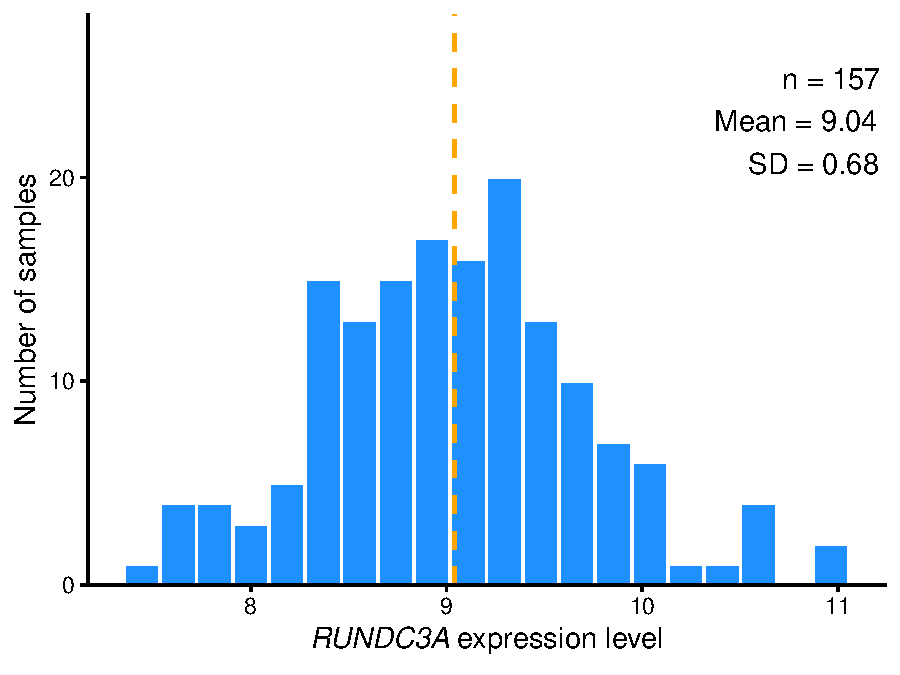
\includegraphics[width=\textwidth]{RUNDC3A_histogram.pdf}
    \caption{}
  \end{subfigure}\hfill
  \begin{subfigure}[b]{0.49\textwidth}
    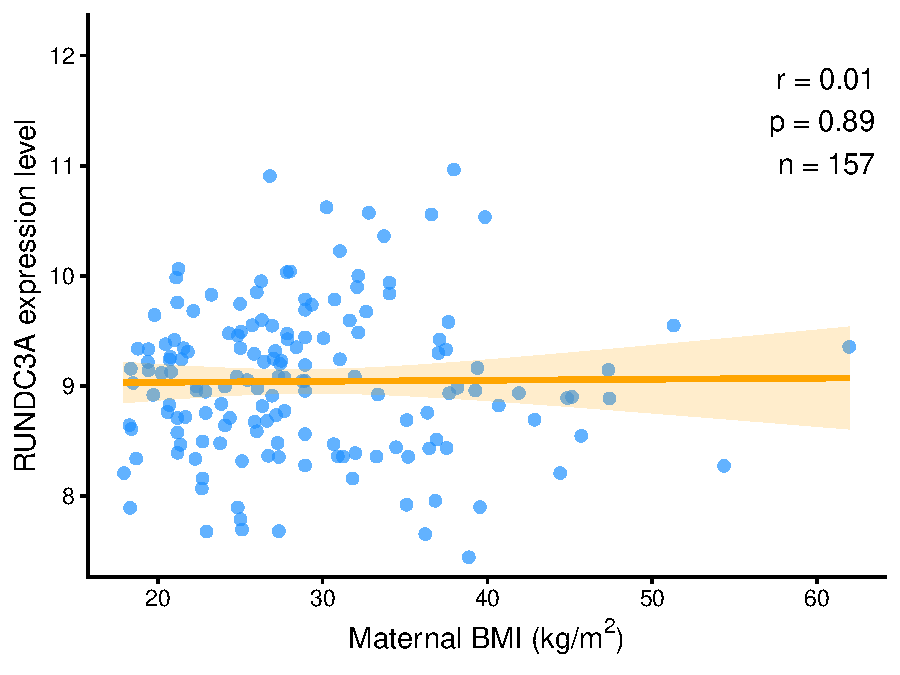
\includegraphics[width=\textwidth]{RUNDC3A_scatter.pdf}
    \caption{}
  \end{subfigure}\\[4pt]
  \begin{subfigure}[b]{0.62\textwidth}
    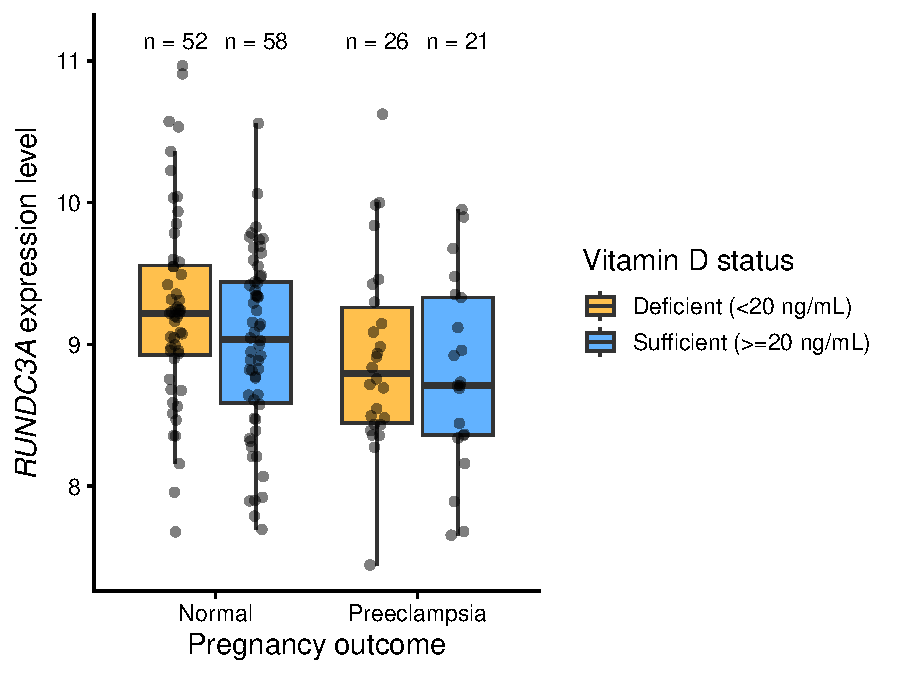
\includegraphics[width=\textwidth]{RUNDC3A_boxplot.pdf}
    \caption{}
  \end{subfigure}
  \caption{\textit{RUNDC3A} expression ($n=157$). (a) Distribution of
  expression; the dashed line marks the mean. (b) Expression against maternal
  BMI with a least-squares line and 95\% confidence band; $r$ is the Pearson
  correlation. (c) Expression by pregnancy outcome and vitamin~D status; points
  are individual women and labels give group sizes.}
  \label{fig:rundc3a}
\end{figure}

% ---- Figure 2: LYN ----------------------------------------------------
\begin{figure}[H]
  \centering
  \begin{subfigure}[b]{0.49\textwidth}
    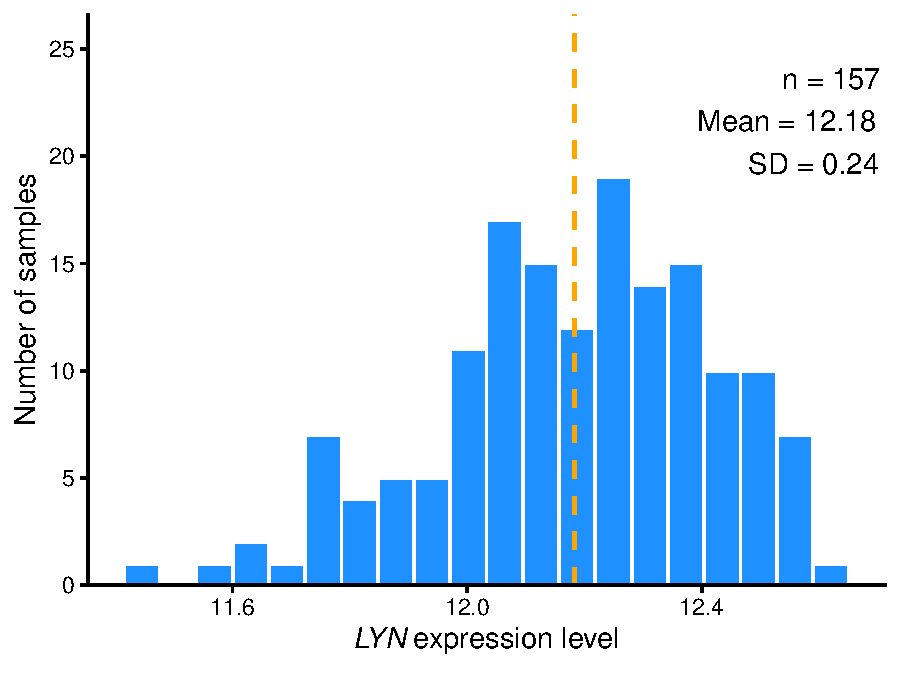
\includegraphics[width=\textwidth]{LYN_histogram.pdf}
    \caption{}
  \end{subfigure}\hfill
  \begin{subfigure}[b]{0.49\textwidth}
    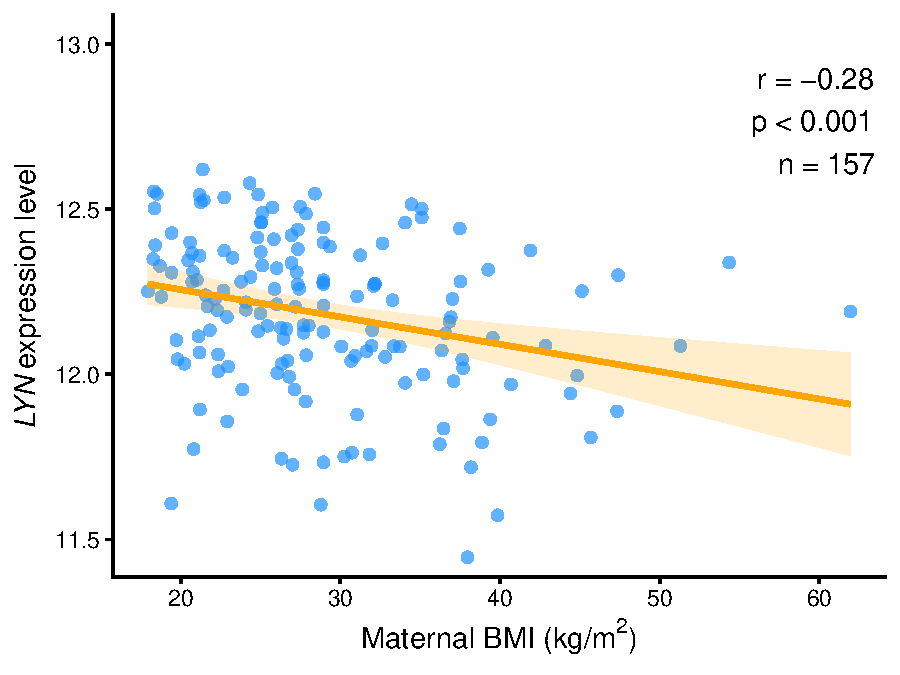
\includegraphics[width=\textwidth]{LYN_scatter.pdf}
    \caption{}
  \end{subfigure}\\[4pt]
  \begin{subfigure}[b]{0.62\textwidth}
    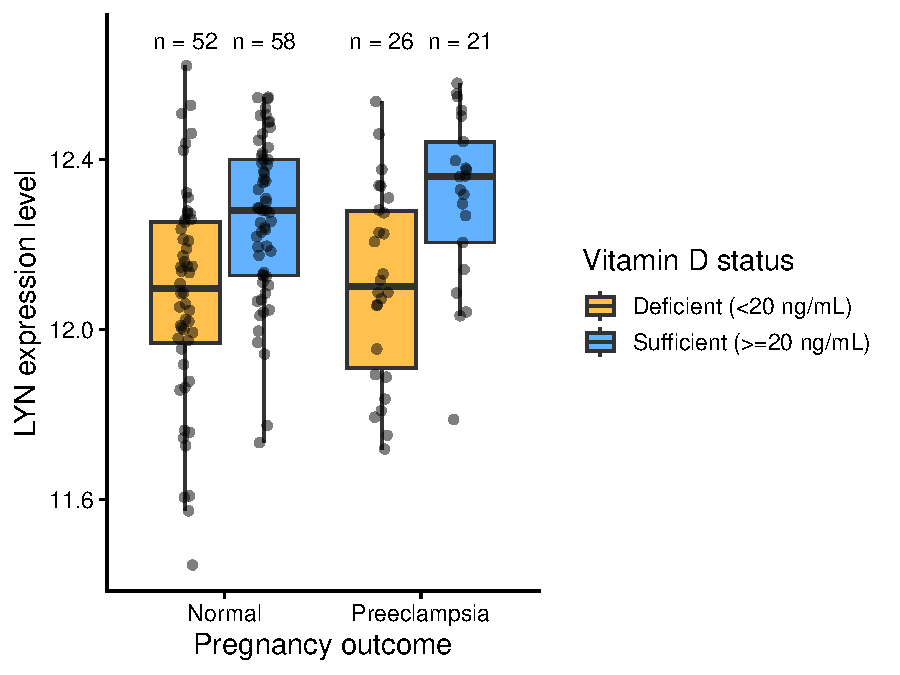
\includegraphics[width=\textwidth]{LYN_boxplot.pdf}
    \caption{}
  \end{subfigure}
  \caption{\textit{LYN} expression ($n=157$). Panels as in
  Figure~\ref{fig:rundc3a}: (a) distribution, (b) relationship with maternal
  BMI, and (c) expression by pregnancy outcome and vitamin~D status.}
  \label{fig:lyn}
\end{figure}

% ---- Figure 3: IGFBP1 -------------------------------------------------
\begin{figure}[H]
  \centering
  \begin{subfigure}[b]{0.49\textwidth}
    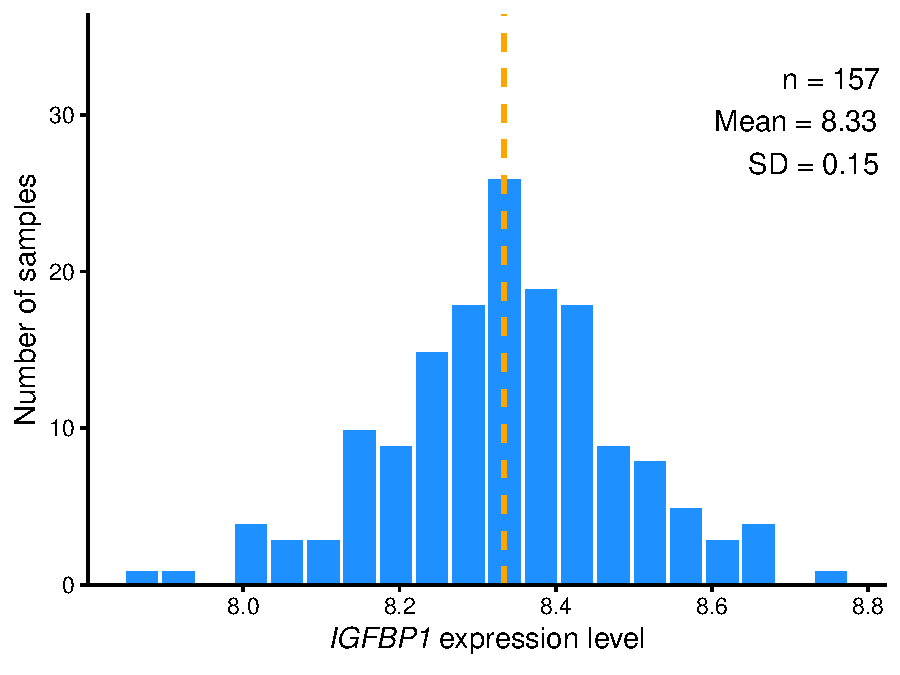
\includegraphics[width=\textwidth]{IGFBP1_histogram.pdf}
    \caption{}
  \end{subfigure}\hfill
  \begin{subfigure}[b]{0.49\textwidth}
    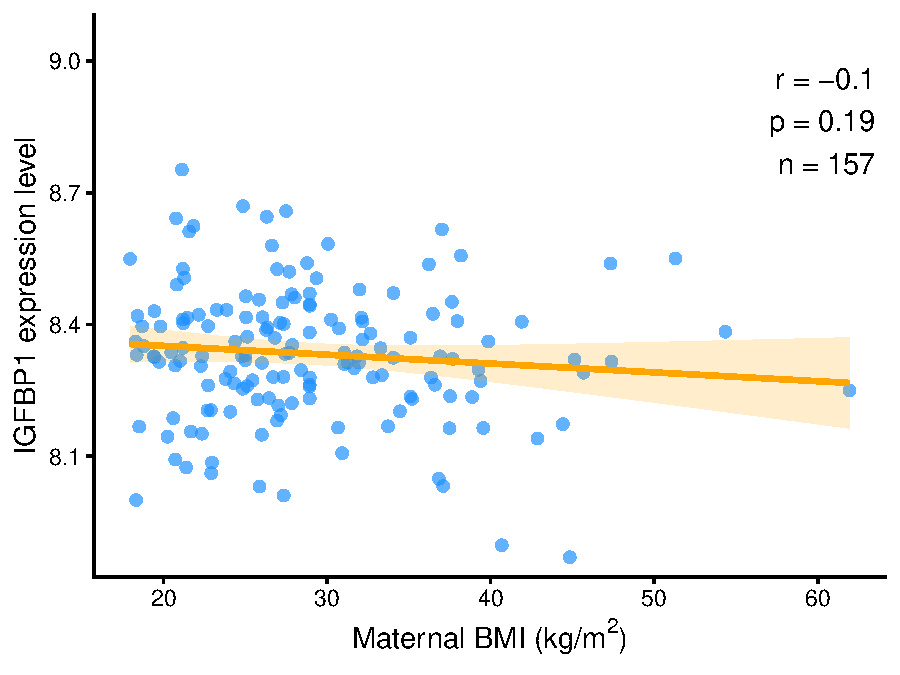
\includegraphics[width=\textwidth]{IGFBP1_scatter.pdf}
    \caption{}
  \end{subfigure}\\[4pt]
  \begin{subfigure}[b]{0.62\textwidth}
    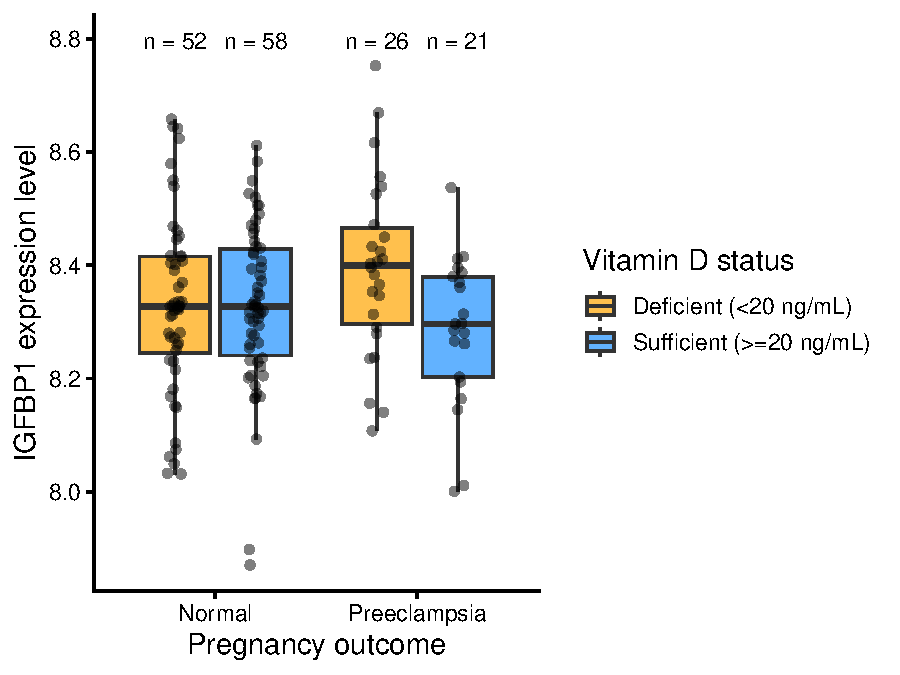
\includegraphics[width=\textwidth]{IGFBP1_boxplot.pdf}
    \caption{}
  \end{subfigure}
  \caption{\textit{IGFBP1} expression ($n=157$). Panels as in
  Figure~\ref{fig:rundc3a}: (a) distribution, (b) relationship with maternal
  BMI, and (c) expression by pregnancy outcome and vitamin~D status.}
  \label{fig:igfbp1}
\end{figure}

\subsection{Heatmap of the 10 most variable genes}
The 10 most variable genes were \textit{UTS2}, \textit{RUNDC3A},
\textit{TMEM176B}, \textit{CEACAM6}, \textit{CLIC2}, \textit{SLC1A5},
\textit{ZNF594}, \textit{ZBTB41}, \textit{CAPZA2}, and \textit{TGM2}.
Clustering on these genes did not separate women by pregnancy outcome. When the
sample dendrogram was cut into two clusters (136 and 21 women), the proportion
who developed preeclampsia was similar in each (30.9\% vs.\ 23.8\%,
$p=0.69$) (Figure~\ref{fig:heatmap}).

\begin{figure}[H]
  \centering
  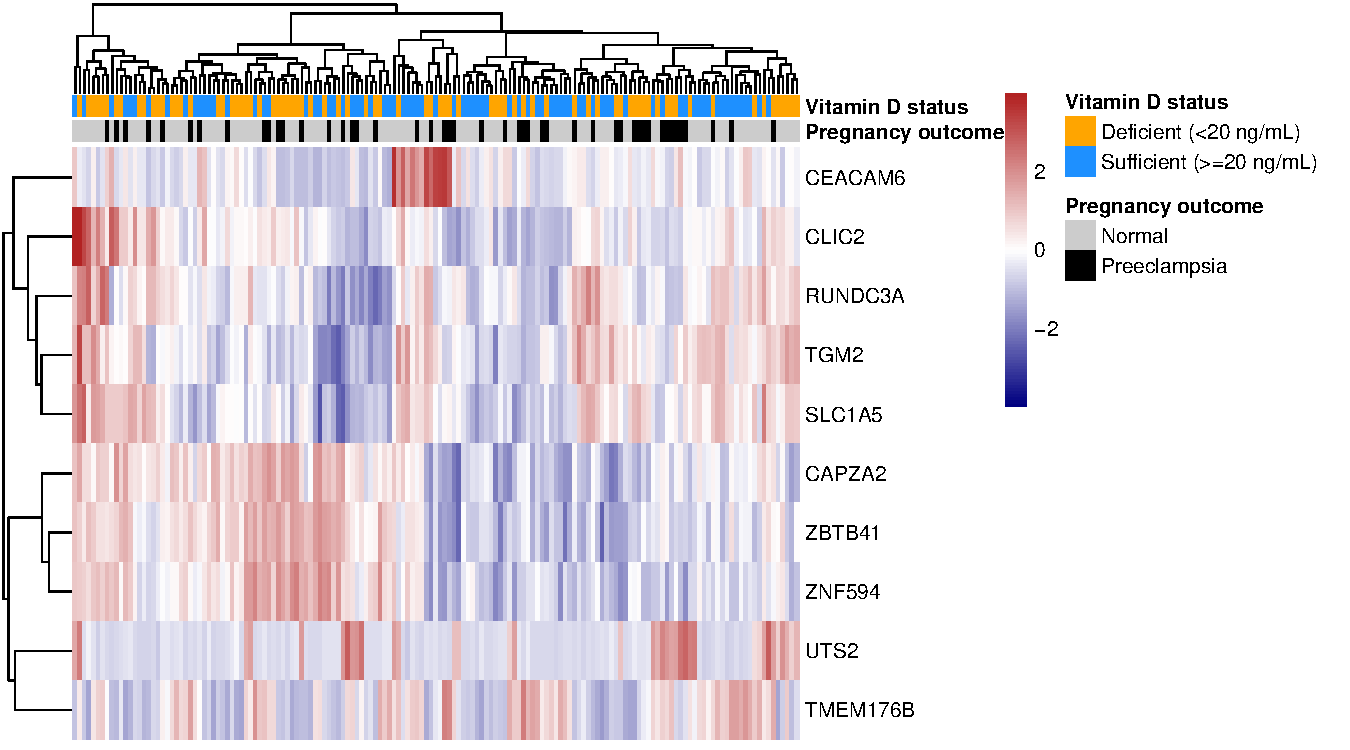
\includegraphics[width=\textwidth]{heatmap.pdf}
  \caption{Hierarchically clustered heatmap of the 10 genes with the largest
  standard deviation across all 157 women. Values are $z$-scores within each
  gene (red above that gene's mean, blue below). Genes (rows) and women
  (columns) are clustered by Euclidean distance with complete linkage. Tracking
  bars show pregnancy outcome and vitamin~D status.}
  \label{fig:heatmap}
\end{figure}

\subsection{Adjusted associations}
After adjusting for each other, preeclampsia was associated with lower
\textit{RUNDC3A} expression ($-0.41$~SD, 95\% CI $-0.75$ to $-0.07$, $p=0.02$),
and vitamin~D sufficiency was also associated with lower \textit{RUNDC3A}
($-0.33$~SD, 95\% CI $-0.65$ to $-0.01$, $p=0.045$). \textit{LYN} showed the
largest effect in the model: vitamin~D sufficient women had expression 0.68~SD
higher (95\% CI 0.38 to 0.98, $p<0.001$), and each 1~SD increase in BMI was
associated with 0.20~SD lower expression (95\% CI $-0.35$ to $-0.04$,
$p=0.01$). No covariate was significantly associated with \textit{IGFBP1},
although vitamin~D sufficiency ($p=0.06$) and BMI ($p=0.06$) were close to the
threshold (Figure~\ref{fig:forest}).

\begin{figure}[H]
  \centering
  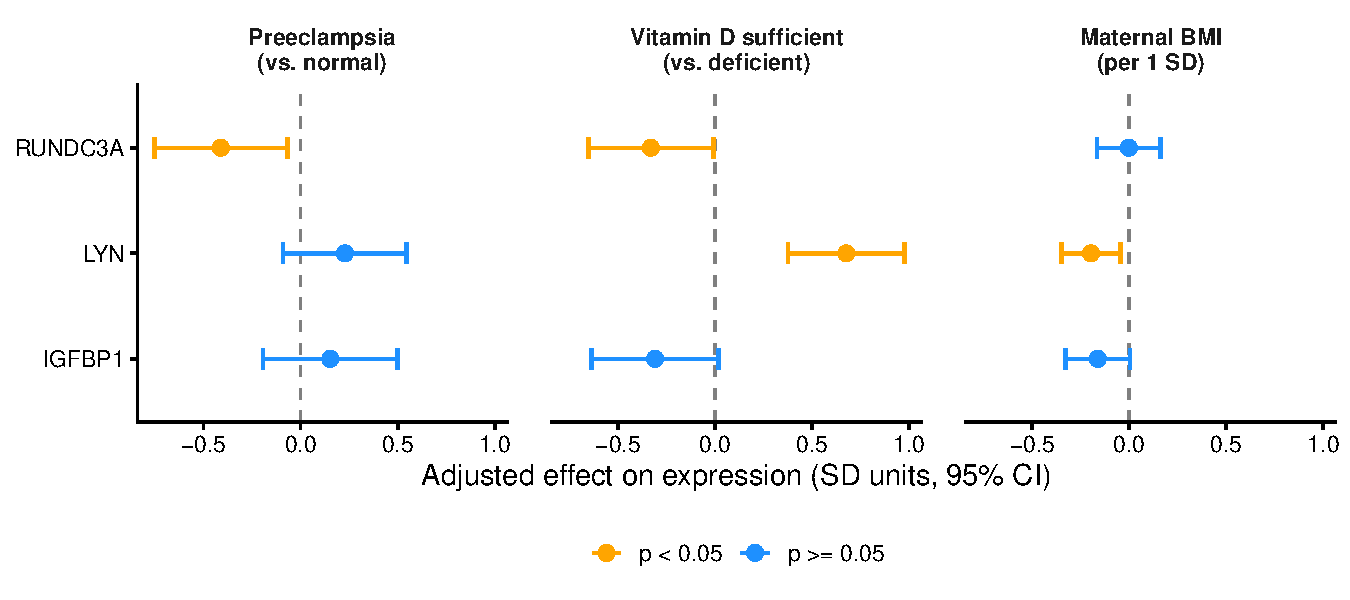
\includegraphics[width=\textwidth]{forest.pdf}
  \caption{Forest plot of adjusted associations with gene expression. For each
  gene, one linear model included pregnancy outcome, vitamin~D status, and
  maternal BMI. Expression and BMI were standardised, so estimates are in
  standard deviations of expression. Points are estimates and bars are 95\%
  confidence intervals; orange marks $p<0.05$. The dashed line marks no effect.}
  \label{fig:forest}
\end{figure}

% =====================================================================
\bibliographystyle{unsrtnat}
\bibliography{references}

\end{document}
